We use \emph{Researching Information Systems and Computing}~\cite{Oates2006} as the
general framework for defining the methodology for our research. On it, Oates describes
six fundamental aspects of research, using the mnemonic `6P':

%\begin{itemize}
    %\item \textbf{Purpose}: The reason for doing the research.
    %\item \textbf{Products}: Its outcomes.
    %\item \textbf{Process}: The sequence of activities.
    %\item \textbf{Participants}: People involved with the research.
    %\item \textbf{Paradigm}: Way of thinking.
    %\item \textbf{Presentation}: Dissemination and explanation of the research.
%\end{itemize}

\paragraph{Purpose}
\label{method:purpose}
A research project needs a well-defined objective to be able
to define what means for it to succeed --- either totally or partially.

First, a \emph{PhD} thesis must \emph{increase the body of knowledge}
of the chosen research area. Second, we want to \emph{solve an existing problem}:
In our case, as discussed in chapter~\ref{chapter:introduction}, we target the
\gls{IDE} research area.

\paragraph{Products}
\label{method:products}
Oates lists five different types of contributions to the body of knowledge, based on
an existing classification from Davis \& Parker~\cite{Oates2006,Davis1997}:

\begin{itemize}
    \item Evidence.
    \item Methodology.
    \item Analysis.
    \item Theories.
    \item Computer-based products.
\end{itemize}

Note that improvements are also considered a contribution under this classification.

For the current thesis, we aim to produce a new computer-based product
for \gls{IDE}, understanding as such novel algorithms and techniques.
The literature review is also a contribution (analysis).

\paragraph{Process}
\label{method:process}

\begin{figure}[htpb]
  \centering
  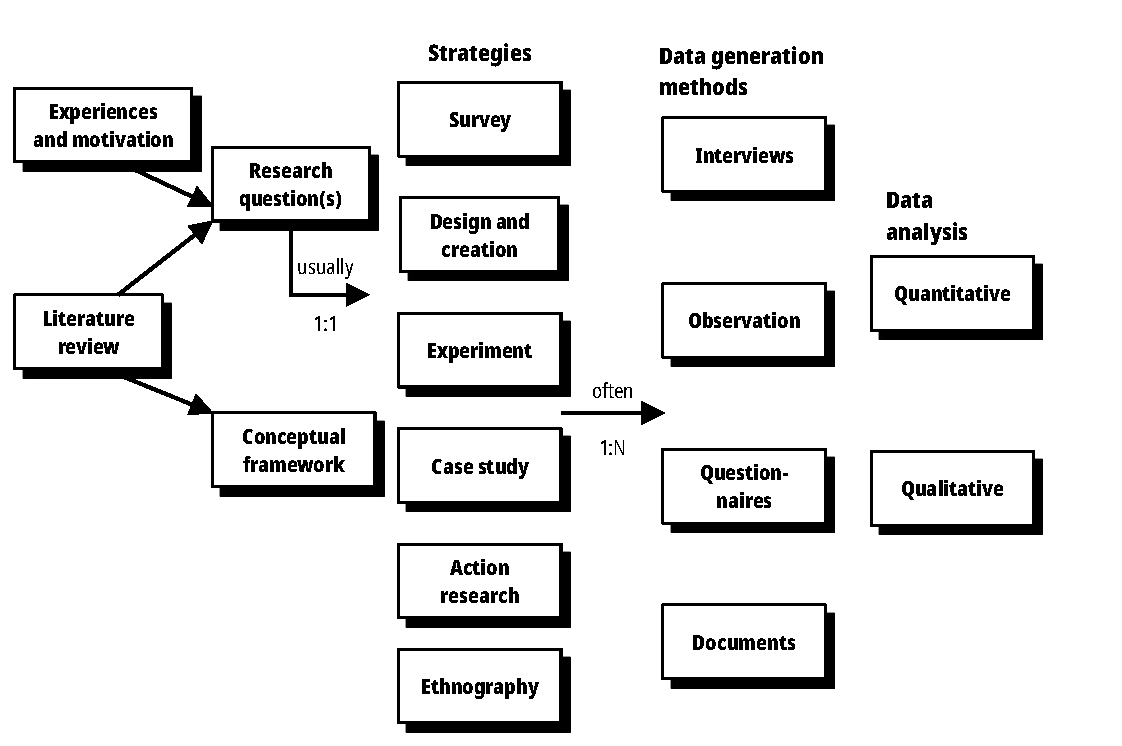
\includegraphics[width=\linewidth]{images/2_methodology/modelo_proceso}
  \caption[Model of the research process]{Model of the research process~\cite{Oates2006}}
  \label{fig:method_process_model}
\end{figure}

Figure~\ref{fig:method_process_model} shows the model of the research process.
The time working at \gls{CERN} and the \emph{Astronomy Department of the University of Geneva}
set up the \emph{experiences and motivations} for this research:
\gls{IDE} on physical measurements,
which have an intrinsic uncertainty. In chapter~\ref{chapter:introduction} we have
introduced the research questions for this thesis.
We will be shortly defining the methodology for the literature review,
the research strategy, the data generation methods, and the data analysis.

\paragraph{Participants}
\label{method:participants}
The direct participants of the current research will be the researcher, the tutor, and
the thesis director. Journal editors and reviewers are indirect participants.

\paragraph{Paradigm}
\label{method:paradigm}
The paradigm is the philosophical model that frames the research.
It defines what the researcher believes on the nature
of reality (\emph{ontology}), how the researcher interacts with
knowledge (\emph{epistemology}), and how knowledge is acquired
(\emph{methodology}). By definition, this framework can not be proven~\cite{Guba1990,guba_competing_1994}.

We can find different classifications of different paradigms depending on
their views on these questions. For instance, Oates and Chua~\cite{Chua1986}
consider three branches:

\begin{itemize}
    \item \emph{Positivism}, where reality is objective and the researcher neutral.
    \item \emph{Interpretative}, where truth is subjective and subject to the context.
    \item \emph{Critic research}, where the social structure is the main focus.
\end{itemize}

Shull \etal~\cite{Shull2008} extends this classification with a fourth paradigm:
the \emph{pragmatism}. In this paradigm, knowledge is evaluated based on its
utility and is considered, in any case, approximate.

Considering our purpose and objective, and given the restricted list of
participants, we will follow the paradigm of \emph{pragmatism} for this research project.

\paragraph{Presentation}
\label{method:presentation}
The main results from our research are compiled into the present thesis
and published in peer-reviewed journals. Drafts have been published in \texttt{arXiv}.
All the relevant source code is publicly available.

\section{Literature review}
\label{sec:method_literature_review}
A systematic mapping study is a process for the exploration of
the situation of a wide research area with a high level of granularity,
allowing us to identify areas in the domain that may be interesting to
explore in more detail~\cite{Kitchenham2007}. Because we are trying to obtain
an overview of the situation of the research on data exploration techniques
and identify where additional work may be required, we have decided to follow this
approach, and, more specifically, the guidelines proposed in
\emph{Systematic Mapping Studies in Software Engineering}~\cite{Petersen2007}.
For completeness, we include in figure \ref{fig:systematicmapping_diagram} the
diagram of the process for a systematic mapping study, as defined by
Petersen \etal.

\begin{figure}[htbp]
    \centering
    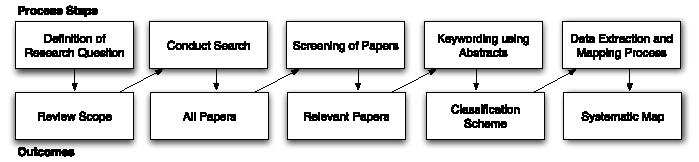
\includegraphics{images/3_mapping/systematicmapping_diagram}
    \caption{The Systematic Mapping process}
    \label{fig:systematicmapping_diagram}
\end{figure}

\section{Research strategy}
\label{sec:method_strategy}
From the list of strategies shown in figure~\ref{fig:method_process_model},
we follow \emph{Design and Creation} and \emph{Experiments}.

\textbf{Design and Creation} is an adequate strategy since we aim for a
computer-based product. The resulting artifacts should be carefully studied and developed and result from a careful engineering approach.
Thus, we follow \emph{Engineering Design}:
    
\begin{displayquote}
  Engineering design is the systematic, intelligent generation and evaluation
  of specifications for artifacts whose form and function achieve stated
  objectives and satisfy specified constraints~\cite{Dym2012}.
\end{displayquote}

Figure~\ref{fig:engineering_design} summarizes the different stages for this method.
We want to emphasize that this method is inherently iterative since each stage
provides feedback to the precedent stages. This work results from many such
iterations: the research plan defined the initial task: \gls{IDE} of raw scientific data.
We performed a systematic literature mapping to identify solution principles and existing problems.
As a result of this literature review, we refined the initial task: data exploration of multiple files with related raw scientific data but incomplete metadata.

\begin{figure}[htbp]
  \centering
  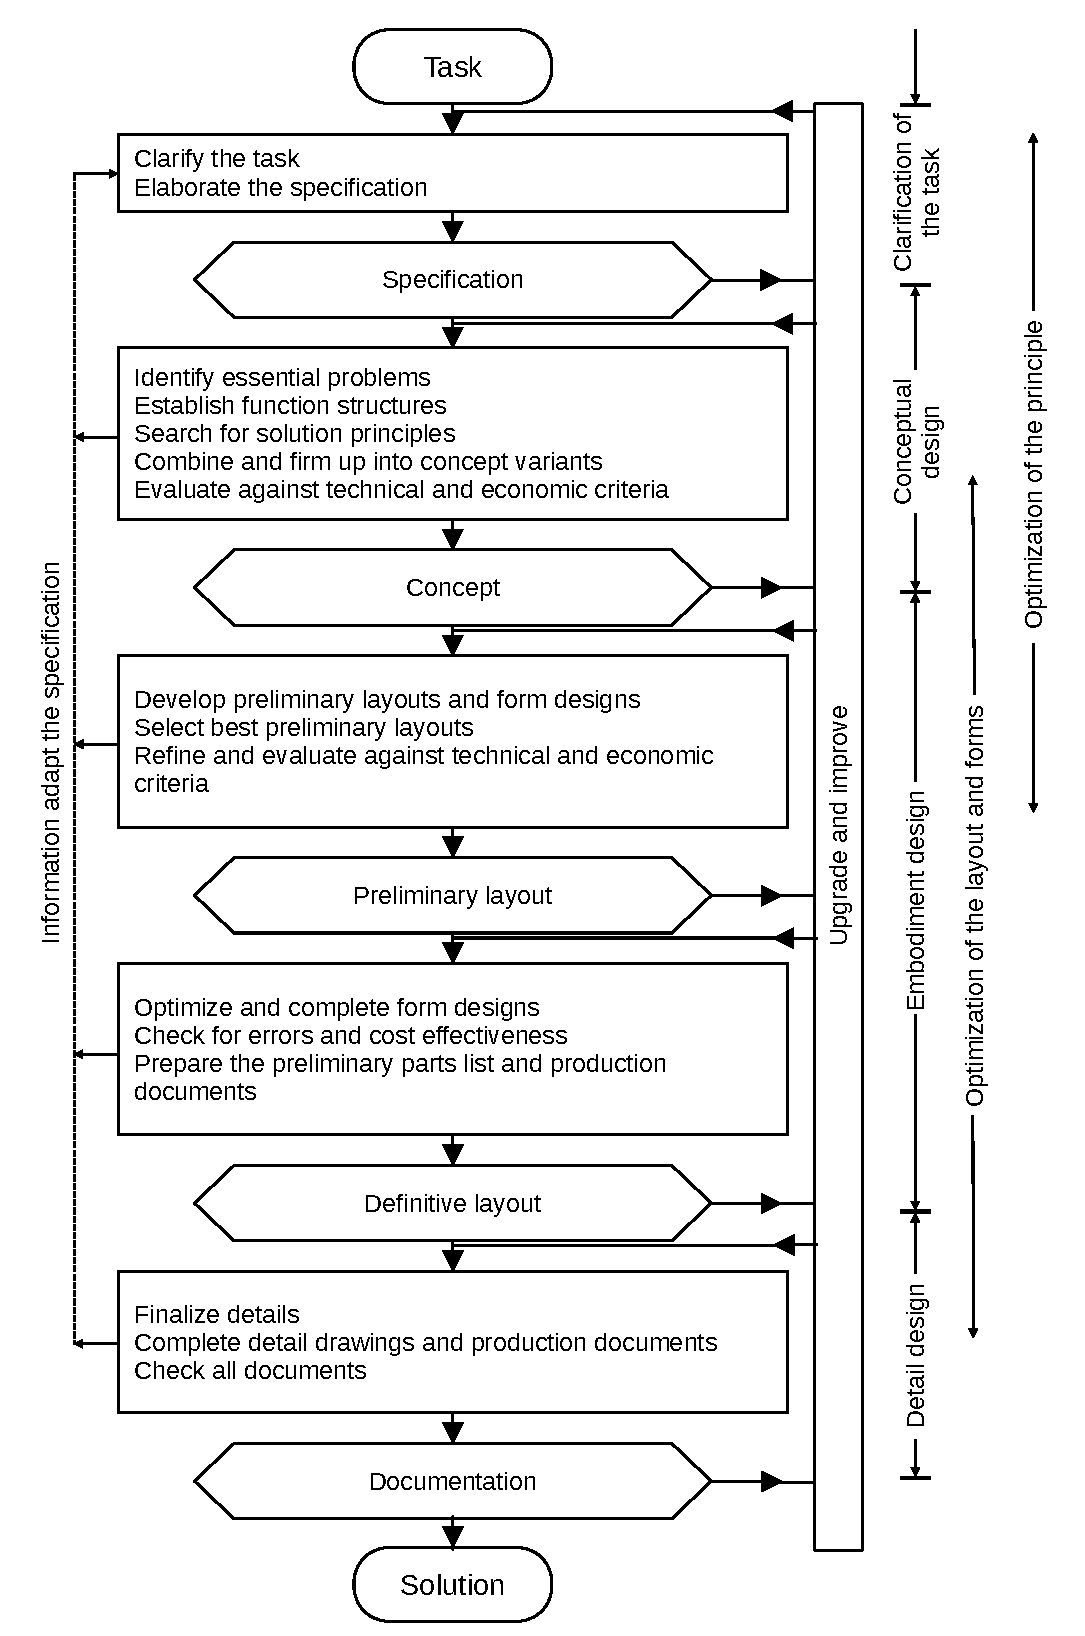
\includegraphics[width=\linewidth]{images/2_methodology/design_process}
  \caption[Engineering Design]{Engineering Design~\cite{Dym2012,Pahl1984}}
  \label{fig:engineering_design}
\end{figure}

\paragraph{Experiments} \emph{Engineering Design} incorporates the development of
multiple preliminary products, which need to be compared and evaluated before refining
them into the final deliverable. Thus, experiments are a central aspect of this method.

%Research question introduction (chap.1), literature review chap.3 (link with methodology here).
%Data generation, observations (experiments), Data Analysis quantitative and qualitative (SOM),
%link with the chapter about discussion/results?
%Documentation is the thesis itself.
%Insist on the feedback loop!

%Task -> Specification -> Concept -> Preliminary chap 4 (bridge, plus preliminary excuse for dead ends)
%Definitive layouts 5 and 6 (presq and som).


\section{Data generation methods}
From the proposed data generation methods, we use \textbf{documents},
such as scientific papers to obtain datasets for the experiments.

With these datasets, we run experiments and \textbf{observe} the results,
using performance metrics to compare different algorithms and their parameterizations.

\section{Data analysis}
We base our comparisons on \textbf{quantitative} metrics: run-time, success rate,
statistical significance, etc.

\section{Open Science}
This research adheres to the \emph{Open Science} principles~\cite{oro44719}.

\begin{itemize}
    \item \textbf{Open Access} Papers are published either on \emph{Open Access} journals,
        or made accessible on pre-print servers.
    \item \textbf{Open Data} The results from our experiments are uploaded to a public server together with the source code.
    \item \textbf{Open Reproducible Research} 
        \begin{itemize}
            \item \textbf{Open Notebooks} Notebooks used to summarize the results are
                included next to the source code.
            \item \textbf{Open Source} The source code is under a permissive free software license
                (MIT\footnote{\url{https://opensource.org/licenses/MIT}}).
            \item \textbf{Reproducibility Guidelines} Even if our results become
            inaccessible, the repositories include a list of the required dependencies so the
            environment can be replicated. The procedure followed to generate our results is documented in appendix~\ref{appendix:presq_benchmarks}.
        \end{itemize}
    \item \textbf{Open Repositories} All the delivered software is in \textsc{GitHub},
        and a copy archived in \href{https://zenodo.org/}{\textsc{Zenodo}}~\cite{zenodo} with an
        associated DOI. Papers are available in pre-print servers such as
        \href{https://arxiv.org/}{\textsc{arXiv}} and
        \href{https://www.techrxiv.org}{\textsc{TechRxiv}}.
\end{itemize}
